% WARNINGS: 
%	    1. You must make sure that PDF output generated from this
%	       template is complete both when displayed with a viewer 
%	       (acroread, for example) and when printed on paper.
%	       LaTeX installations vary greatly and therefore it might 
%	       not be possible to get all proposals to come out 
%	       correctly with a single text page layout. 
%	       In some cases you will have to adjust the 
%	       \topmargin=-7mm command in the template to center the 
%	       text vertically in the page.  
\documentclass[12pt,a4paper]{article} 
\usepackage{times}
\usepackage{graphics,graphicx}
\usepackage[update,prepend]{epstopdf}
\usepackage[innercaption]{sidecap}
\usepackage{subcaption}
\usepackage{amssymb, amsmath}	       
\usepackage{xspace}				
\usepackage{natbibspacing, natbib}
\usepackage{aas_macros}
\usepackage{wrapfig}
\usepackage{floatrow}

\newcommand{\ncrit}{\mbox{$n_{\rm crit}$}\xspace}
\newcommand{\comol}{$^{12}$CO\xspace}
\newcommand{\Lsun}{\mbox{L$_{\odot}$}\xspace}
\newcommand{\LIR}{\mbox{$L_{\rm IR}$}\xspace}
\newcommand{\LFIR}{\mbox{$L_{\rm FIR}$}\xspace}
\newcommand{\rarr}{$\rightarrow$}
\newcommand{\aco}{\mbox{CO($J$=1\rarr0)}\xspace}
\newcommand{\bco}{\mbox{CO($J$=2\rarr1)}\xspace}
\newcommand{\cco}{\mbox{CO($J$=3\rarr2)}\xspace}
\newcommand{\eco}{\mbox{CO($J$=5\rarr4)}\xspace}
\newcommand{\rot}[3][HCN]{\mbox{#1($J$=#2\rarr#3)}\xspace} 
% default HCN; usage \rot[HCN]{3}{2} or \rot[\hcop]{4}{3}
\newcommand{\ahcn}{HCN($J$=1\rarr0)\xspace}
\newcommand{\dhcn}{HCN($J$=4\rarr3)\xspace}
\newcommand{\hcop}{HCO$^+$\xspace}
\newcommand{\ahcop}{\mbox{HCO$^+$($J$=1\rarr0)}}
\newcommand{\dhcop}{HCO$^+$($J$=4\rarr3)\xspace}
\newcommand{\Lp}[1][CO]{\mbox{$L^{\prime}_\textrm{\fontsize{8pt}{12pt}\selectfont{#1}}$}}
\newcommand{\LpU}{\mbox{K\,\,km\,\,s$^{-1}$\,\,pc$^2$}}
\newcommand{\kms}{km\,s$^{-1}$\xspace}
\newcommand{\pmOne}{\mbox{$^{-1}$}\xspace}
\newcommand{\Fig}[1]{Fig.~\ref{fig:#1}}
\newcommand{\Eq}[1]{Equation~\ref{eq:#1}}

%Compact BIB%%%%%%%%%%%%%%%%%%%%
\citestyle{aa}	
\bibliographystyle{apj_w_etal_3auth}

\usepackage{paralist}

\renewenvironment{thebibliography}[1]{%
%\section*{\refname}%
%  {\normalsize {\textbf{References:}}}
  \let\par\relax\let\newblock\relax%
  \inparaitem[{[}1{]}]}{\endinparaitem}
%%%%%%%%%%%%%%%%%%%%%%%%%%%%%


%%%%%%%%%%%%%%%%%%%%%%%%%%%%
%%%%%% Page dimensions %%%%%
%%%%%%	DO NOT CHANGE  %%%%%
%%%%%%%%%%%%%%%%%%%%%%%%%%%%

\textheight=247mm
\textwidth=180mm
\topmargin=-7mm
\oddsidemargin=-10mm
\evensidemargin=-10mm
\parindent 10pt

\renewcommand\floatpagefraction{.9}
\renewcommand\topfraction{.9}
\renewcommand\bottomfraction{.9}
\renewcommand\textfraction{.1}
% between fig
\setlength{\textfloatsep}{10pt plus 1.0pt minus2.0pt}
\setlength{\floatsep}{10pt plus 1.0pt minus 2.0pt}
\setlength{\intextsep}{10pt plus 1.0pt minus 2.0pt}
\setlength{\parskip}{0.01em}
\usepackage[small,tiny,compact]{titlesec}

\begin{document}
\pagestyle{plain}
\pagenumbering{arabic}
 
\begin{center}
{\large{\bf
{ 
Dense gas properties in a strongly-lensed wet merger: bridging the gap between local ULIRGs and high-z systems}
}}
\end{center}
\vspace{-0.545em}
\centerline{\normalsize{\bf PI: 
{T. K. Daisy Leung}}} 
%%%%%%%%%%%%%%%%%%%%%%%%%%%%%%%%%%
\vspace{0.1em} {\bf Missing link between mergers/ULIRGs and their high-z analogues} 
Ultraluminous infrared galaxies (ULIRGs: \LIR$\geq$10$^{12}$\Lsun) have been
regarded as analogues of high-redshift (z) starbursts given the
similarities in their interstellar medium (ISM; e.g. \LIR/\Lp).
As such, detailed studies 
of ULIRGs are important 
to gain more detailed insight into the early universe and in studies of galaxy evolution over cosmic time.
While mergers are believed to play an important role in giving rise to these dusty galaxies
(e.g. Sanders \& Mirabel 1996), merger-induced effects on the physical mechanisms and chemistry 
that drive the starburst (SB) and active galactic nucleus (AGN) activities on small scales are still unclear.

While the ISM in local ULIRGs has been studied in great detail,
forming a rich inventory of molecular transitions that serves as the template for 
studying high-z galaxies 
\citep[e.g.,][]{Rangwala15a}, a wide knowledge gap persists
between $z$=0 and the epoch when most stars are formed in the universe ($z$$\sim$2). 
Here we aim to bridge this gap by testing
local correlations and properties at moderate redshifts 
% Understanding galaxy populations at an epoch when
% the build-up of stellar mass 
% is steeply rising ($z$$\sim$0.3-1) is critical.
by observing the 
dynamical structure and properties of the ISM of
the quadruply lensed galaxy RXJ1131-1231 (henceforth RX1131) and its dust-obscured 
companion at $z_{\rm CO}$$\sim$0.65 (\Fig{HST}).

\noindent {\bf Molecular gas in AGN/SB} 
Extreme star formation rates (SFRs) in ULIRGs and their high-z analogues are a natural consequence of either gas 
being converted into stars more efficiently and/or their high molecular gas fractions, whch
would lead to fragmentation of giant star-forming clumps and turbulent conditions 
due to gravitational instability. Indeed, observations at $z$=1--2 have found gas clumps of
size $\sim$few kpc \citep{Swinbank12a, Swinbank12b}, which are much bigger than 
those in normal star-forming galaxies. Therefore, resolving the gas dynamics 
on sub-kpc scales is important to understand the 
mechanism and physical processes responsible for 
the different star-formation modes in normal galaxies and ULIRGs. % at earlier epochs.
% star-formation and how the ISM conditions 
% are related to the SB in ULIRGs at this epoch.

While \comol emission traces the total molecular distribution and dynamics,
high-dipole moment molecules such as HCN and \hcop are expected to trace the 
%properties of the 
denser, actively star-forming gas. Indeed, a tight correlation between \ahcn and \LIR 
(a proxy for SFR) has been found in nearby galaxies and local giant molecular 
clouds (GMCs; \citealt[hereafter GS04]{Gao04a}; \citealt{Wu05}), 
suggesting HCN is a faithful tracer of the star-forming dense gas.
However, higher-$J$ transitions (e.g. $J$=4\rarr3) 
have also been suggested to be better proxies
of the star-forming gas since they
trace the much denser gas (n$\gtrsim$10$^5$-10$^7$ cm$^{-3}$) that is 
thought to be the immediate fuel for SF in turbulent GMCs \citep{Shirley03a, KM05}.
This is supported by the linear correlations found in 
\LIR-\Lp[\dhcn] and \LIR-\Lp[\dhcop] \citep[]{Zhang14a}.
Since the 
ground state lines are redshifted to frequencies beyond the spectral coverage of ALMA
at $z$$>$0.06, it is important to establish diagnostics using these mid-$J$ lines to 
study distant galaxies.
Due to the difference in abundances and excitation conditions of HCN and \hcop
in star-forming versus AGN regions, the line 
% ratios \ahcn/HCO$^+$($J$=1\rarr0) \citep{Kohno05a, Imanishi10, Izumi13a} and
ratio \dhcn/\dhcop has been 
proposed as
%  diagnostic tools 
a diagnostic tool to reveal deeply buried AGNs at the cores of ULIRGs \citep{Imanishi14a, GB14a, Viti14a, 
Izumi16a, Imanishi16a}.
% separate emission originating from AGN and SB
% Recent studies have
% extended this diagnostic to using the J=4\rarr3 transitions 
%\citep{Imanishi14a, GB14a, Viti14a}, 
% where an elevated line ratio is seen in AGNs, suggesting
% it can be used to reveal deeply buried AGNs at the cores of ULIRGs \citep{Izumi16a, Imanishi16a}.

Prior to ALMA, studies using dense gas tracers were largely limited 
to the local universe ($z$$\lesssim$0.1) with only five detections
%IR-luminous lensed galaxies detected 
at $z$$\gtrsim$0.3
(e.g., \citealt{Riechers07a, Riechers10a, Wagg05a, Gao07a}).
Moreover, none of these 
spatially resolve the emission, rendering it difficult 
to draw more detailed conclusions on the dense gas properties of galaxies at high z. 
Even with ALMA, such studies will remain challenging, but by combining 
the magnification provided by gravitational lensing with the exceptional spatial resolution and sensitivity of ALMA, 
studies
of dense molecular gas in distant galaxies are now possible, as proposed here.

%%%%%%%%%%%%%%%%%%%%%%%%%%%%%%%%%% 
\noindent {\bf Science Target RXJ 1131-1231: a demonstrative case at high-z}
% \vspace{-0.6em}

\begin{figure}[!tbhp]
\hspace{-1em}
\centering
\floatbox[{\capbeside\thisfloatsetup{capbesideposition={right,center},capbesidewidth=0.395\textwidth}}]{figure}
[\FBwidth]
{\hspace{-0.5em}
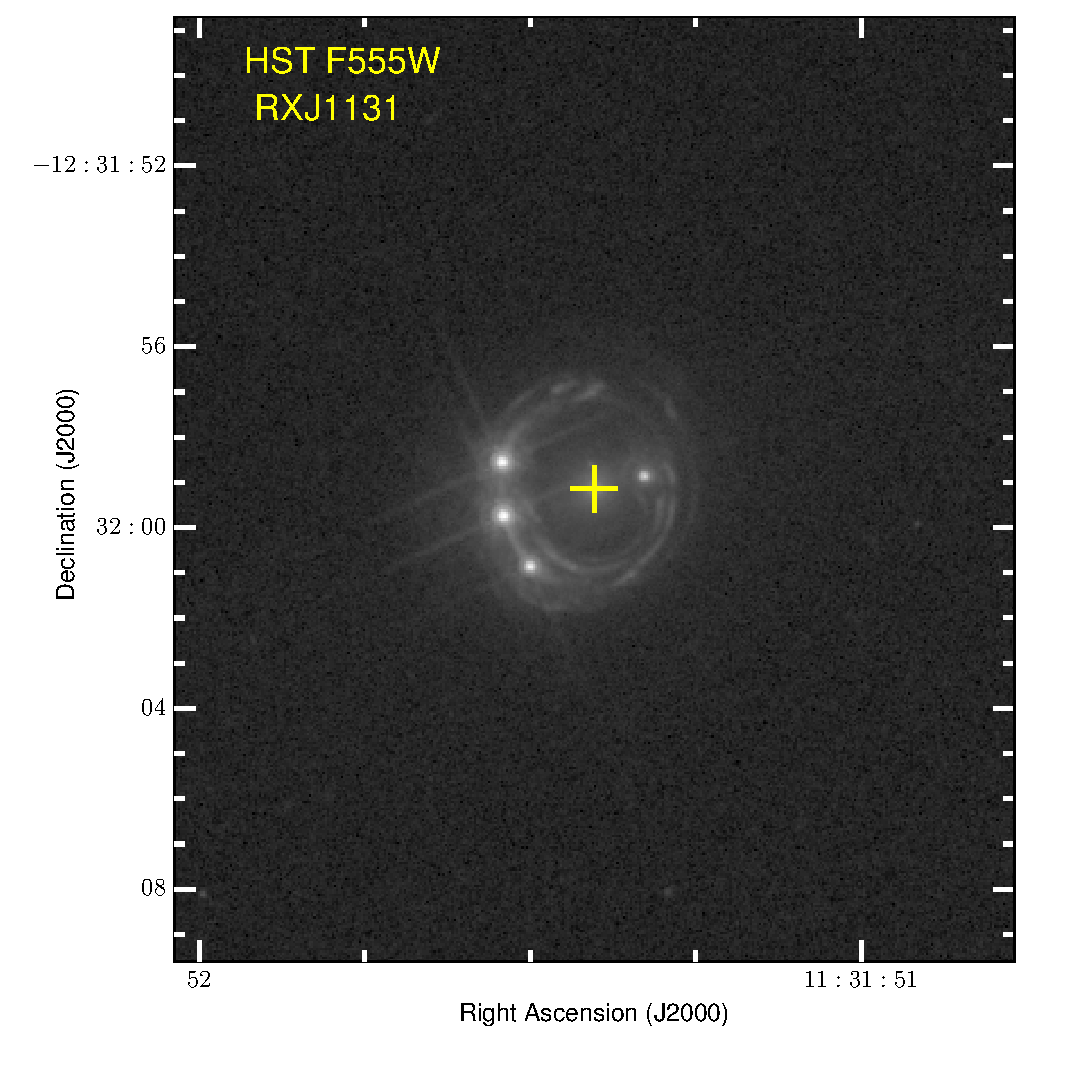
\includegraphics[trim= 10 20 15 0, clip, scale=0.278]{Fig/F555W}
\hspace{-1.325em}
\includegraphics[trim= 10 0 0 5, clip, scale=0.345]{Fig/Manipulate_figsCROP}
\vspace{-1.0em}
}
{
\hspace{-0.45em}
\caption{\fontsize{10pt}{12pt}\selectfont{\textbf{Stellar light distribution in the AGN host galaxy of RXJ 1131-1231 
and its reconstructed source plane
morphology.}
{\em Left:} The rest-frame UV emission (tracing recent star-formation) 
is lensed into an almost complete Einstein ring with diameter $\sim$3.8". 
{\em Right:} Lens modeling of the optical emission identifies complex structures in the host galaxy and
an optically faint companion (white component as indicated by the blue arrows; \citealt{Claeskens06a}), 
which we have recently confirmed by lens-modeling \bco emission detected with NOEMA
(\Fig{combine}; Leung \& Riechers, in prep.). 
Here we propose to study
the ISM conditions in this AGN-starburst merger with finer
detail than otherwise possible with current facilities. 
}
\label{fig:HST}}}
\vspace{-0.8em}
\end{figure}
RX1131 is a quadruply imaged AGN with its host galaxy lensed 
into a partial Einstein ring (\Fig{HST}). 
HST observations (rest-frame UV) have revealed distinct emission 
from recent star-formation (lensing arcs) and from the AGN (bright knots) in the background galaxy \citep{Sluse03a},
demonstrating the great potential for probing its
ISM conditions in detail. Lens modeling carried out on optical images shows
that the AGN resides in a star-forming region of size $\sim$1 kpc
% $\sim$0.15" (without lensing magnification)
in its host galaxy, which itself is 7 kpc across, % $\sim$ 1 " (without lensing)
and made it possible to identify
seven distinct structures in the source plane (\Fig{HST}). 
A companion galaxy of size $\sim$700 pc across was also identified at $\sim$2.4 kpc away
from the AGN host galaxy
in the HST observations \citep{Brewer08a}.
We recently confirmed that both galaxies are at the same redshift by detecting their 
\rot[CO]{2}{1} emission and lens-modeling their gas distribution 
in velocity space (\Fig{combine}f), verifying
that both are gas-rich (Leung \& Riechers, in prep.). 
Our SED modeling of the dust continuum emission up to 250\,$\mu$m finds $L_{\rm IR}\sim6\times$10$^{12}$\Lsun 
(corrected for lensing). Hence, this target is a gas-rich ULIRG merger at $z$$\sim$0.7 caught in the act. 

%%%%%%%%%%%%%%%%%%%%%%%%%%%%%%%%%%
\noindent {\bf Proposed Observations and Science Goals}
Here we propose to map (1): \eco at 0.15" resolution ($\sim$500pc at $z$$\sim$0.7 in the source plane) and 
(2): \dhcn and \dhcop emission and the underlying continuum at 0.7" resolution (2.5 kpc in the source plane).
The continuum will provide additional constraint on the Rayleigh-Jeans tail of the 
dust emission, which is currently constrained by four photometric data. 
This will reduce the uncertainties on the the gas-to-dust ratio, dust temperature(s), dust mass,
and its spatial extent (and thus the surface density of the SFR) .
These quantities are important for investigating how the ISM
varies as galaxies evolve across cosmic time.
In conjunction with the large set of ancillary data 
(from rest-frame UV to radio wavelengths, including our recent observations of \bco and CO\,$J$=3\rarr2), our
proposed observations are designed to investigate:

\underline{\bf(1) Dynamics and kinematics}
Our recently obtained \bco data shows an asymmetric double-horned line profile (\Fig{combine}a). Given
the 1$^{\rm st}$ moment map and the observed velocity gradient
across the source plane in our model (\Fig{combine}d, f), this is indicative of
a kinematically ordered %(reminiscent of a rotating disk) 
galaxy, but its emission has been lensed differentially. 
Limited by the spatial resolution of this data, it is not possible to infer the true 
kinematics due to beam smearing.
Furthermore, the unusually high velocity dispersion 
($\gtrsim$400\kms) in the central region (\Fig{combine}e) hints at 
perturbations from the AGN, 
internal turbulence due to interactions with the companion,
and/or instability due to the huge gas reservoir.
Therefore, higher-resolution \eco imaging, as proposed here, is needed
to distinguish 
between a merger-driven and a turbulent clumpy disk starburst.

The requested resolution for \eco is critical
as it allows us to obtain a detailed
dynamical lens model of the system and therefore probe structure at sub-kpc scales
(typical size of high-z GMCs), as well as enables us 
to compare the spatial distributions of star-forming gas clumps 
with recent star-formation (from HST).
Such comparisons are the key for understanding different processes
that regulate the SB
in ULIRGs/mergers and examining how they differ from other galaxy populations.
% kinematics
We will also measure the linewidths of the very dense gas (traced by HCN and \hcop), 
the highly excited warm gas (traced by CO\,$J$=5\rarr4), and the more-extended, less-perturbed 
molecular gas (traced by low-$J$ CO) at various regions within the AGN host galaxy 
to constrain the kinematics and relative mass-fractions of different gas phases, 
which are indicative of the evolutionary stage of this galaxy.

\underline{\bf(2) Line ratios and the AGN/SB diagnostic}
Aided by lensing, we will be able obtain kinematical information on spatial 
scales smaller than the beam, as seen in our \bco data (\Fig{combine}c, d), thereby
enabling us to probe the physical properties of
the inner molecular disk near the AGN of RX1131. 
Recent studies find that the \dhcn/\dhcop line ratio is enhanced 
in the circumnuclear disk (CND) near AGNs, and falls off with distance from the CND
\citep{GB14a,Imanishi16a}. At the proposed resolution, we will 
resolve the line emission originating near the AGN and that from the spatially extended 
SB regions ($>$kpc scales) in the host galaxy. By measuring spatial variations in 
this line ratio, we will assess its utility 
as an AGN/SB diagnostic (\Fig{AGNSB}) at $z$$\sim$0.7.
Since the HCN vibrational line (v$_2$=1;$J$=4\rarr3) falls within the targeted frequency range, 
we will use it to independently constrain the radiation properties of the AGN environment,
given that this line is excited by infrared pumping of
the same radiation field associated with the AGN that causes the elevated \dhcn/\dhcop
\citep{Sakamoto10a,Imanishi13a}.
The proposed spatial resolution is also necessary for
a detailed lens modeling of each emission line, enabling measurements of reliable line 
ratios without significant uncertainties due to differential lensing.
\begin{figure*}[!tbph]
\vspace{-0.8em}
\hspace{-0.65em}
\centering
\floatbox[{\capbeside\thisfloatsetup{capbesideposition={right,center},capbesidewidth=0.625\textwidth}}]{figure}
[\FBwidth]
{\includegraphics[trim=15 0 5 10, clip, width=0.35\textwidth]{Fig/izumi15}}
{
\hspace{-1.35em}
\vspace{-1.15em}
\caption{ \fontsize{10pt}{12pt}\selectfont {\textbf{\dhcn/\dhcop as AGN/SB diagnostic.}
Differences in line ratios between local AGNs, SBs, and (U)LIRGs with buried AGNs suggest
that \dhcn/\dhcop can be used as a diagnostic tool to distinguish between
the energy source from an AGN and starbursts,
where an elevated line ratio is seen in AGN-dominated regions relative to starbursts.
Such diagnostics depend heavily on the spatial resolution, as demonstrated by the
measurements taken with APEX (empty circle) and ALMA (filled circles) in NGC1068.
We here propose to spatially resolve this line ratio within RX1131
%  and obtain
% measurements toward the AGN and the extended SB regions 
in order to 
% investigate spatial variations and 
assess its utility as an AGN/SB diagnostic at high redshift.
(Figure taken from \citealt{Izumi16a})}
\label{fig:AGNSB}}
}
\vspace{-0.905em}
\end{figure*}

% 
% mounting supporting evidence for such elevated
% HCN emission at the centers of local Seyfert galaxies has been accumulated (e.g., Kohno
% et al. 2001; Imanishi et al. 2006; Krips et al. 2008), giving an empirical AGN diagnostic.
%
%mounting evidence that HCN lines can be
%overluminous with respect to the lines of other dense molecular
%gas tracers, like HCO+, in the circumnuclear disks of
%Seyferts (Kohno et al. 2001; Usero et al. 2004; Kohno 2005).
%A significant percentage of luminous and ultraluminous infrared
%galaxies (LIRGs and ULIRGs) has also been reported
%to show high HCN/HCO+ intensity ratios (Graci�-Carpio et al.
%2006; Imanishi et al. 2006, 2007).
% 
%  More recently, spatially resolved ALMA observations
% of HCN(4-3) and HCO+(4-3) at the CND of NGC 1068 at a ?50 pc resolution reveal
% that the HCN(4-3)/HCO+(4-3) line ratios are indeed highly elevated at the CND but
% not significantly at the very position of the active nucleus (Garc??a-Burillo et al. 2014;
% Viti et al. 2014). This indicates that HCN enhancement is not simply caused by X-ray
% irradiation. Recent HCN(4-3)/HCO+(4-3) measurements of the high-luminosity
% type-1 AGN NGC 7469 (Izumi et al. 2015a) with LX = 2 � 1043 erg s?1
% suggest that the
% degree of HCN enhancement is not very different from that in NGC 1097 (Izumi et al.
% 2013), a much lower luminosity type-1 AGN (LX = 7�1040 erg s?1
% ), also adding further
% evidence against the XDR origin of enhanced HCN in AGNs (see also Mart??n et al. 2015).
% 
% physical properties
In addition, we will use spatially resolved line ratios of HCN/CO and \hcop/CO within RX1131
as proxies of its very dense (cores; $\sim$10$^5$-10$^7$ cm$^{-3}$) versus the less dense (clumps; $\sim$10$^4$
cm$^{-3}$) gas content and their spatial distributions as a function of distance from the AGN. 
This will enable us to use relations such as HCN/CO-\LIR to investigate the main driver 
of the enhanced SFRs in ULIRGs (e.g., if they all tend to have high dense gas fraction toward their central regions).
% An increase in line ratios between high-density and low-density molecular gas tracers (e.g. HCN/CO) 
%with increasing infrared luminosity suggests that the main driver of the enhanced SFR
%is the molecular gas density distribution, in agreement with the observations that ULIRGs
%host large reservoirs of dense molecular gas in their
%central regions. 
Measuring the gas kinematics and variations 
in these line ratios will thus provide clues on how galaxy 
interactions drive gas into inner disks to initiate SB/AGN activity and 
how the excitation of gas differs from 
normal star-forming galaxies.
% CO SLED
We will also combine \eco with our existing \bco and CO($J$=3\rarr2) 
data to constrain the gas density ($n_{\rm H_{2}}$) 
and kinetic temperature by performing large velocity gradient (LVG) modeling. 

\underline{\bf(3) The SK Law for dense gas}
The Schmidt-Kennicutt (SK) relation (%``Star-formation law"; 
$\Sigma_{\rm SFR}$$\propto$$\Sigma^N_{\rm gas}$; \Fig{SF})
is one of the key ingredients
for theoretical models of galaxy evolution since it encodes the physical processes and timescales
regulating star-formation and their dependence on the ISM 
(e.g., \citealt{Narayanan14a}).
However, the surface density of gas at high densities ($n$$\gtrsim$10$^5$cm$^{-3}$; 
$\Sigma_{\rm dense}$)
is poorly constrained 
for high-z galaxies due to the lack of 
{\em spatially resolved} observations of the much weaker emission 
from high critical density tracers.
It is therefore unclear how the power-law index of the SK relation should change depending on
the critical density of the tracer used to probe the SF gas \citep[e.g.,][]{KT07a}
and how the SFR surface density could differ between normal galaxies and in mergers
depending on their global dynamical timescales.
At the proposed resolution, we will spatially resolve, for the first time,
the {\it true SK relation} by measuring the {\em dense} gas surface density 
in a high-z merger, down to the size scale of star-forming gas clumps. 
This will provide crucial constraints on the conditions for star-formation at high redshift.

\medskip
\noindent In summary, our proposed observations provide an exceptional opportunity to investigate
the physical properties and dynamical structures of different gas phases in the ISM 
of a distant merger at exquisite detail. 
This will also demonstrate the capabilities of ALMA to % mapping 
utilize these much fainter
high-dipole moment molecules as routine tracers to 
study star-formation at earlier cosmic epochs.

\begin{figure*}[!tbph]
\vspace{-0.55em}
\centering
\floatbox[{\capbeside\thisfloatsetup{capbesideposition={right,center},capbesidewidth=0.625\textwidth}}]{figure}
[\FBwidth]
{
\includegraphics[trim=0 0 0 0, clip, angle=-90, width=0.25\textwidth]{Fig/SFRSD}} 
{
\hspace{-0.54em}
\caption{ \fontsize{10pt}{12pt}\selectfont{
\textbf{Schmidt-Kennicutt relation for dense gas.}
While constraints on the power-law index from gas of different densities are important for 
star-formation models, current studies only have constraints
on gas of densities below \ncrit of the ground state transition of HCN (\ncrit$\sim$10$^{4}$).
These studies are also largely limited to measurements of local galaxies \citep{GB12a}. 
Our proposed observations will, for the first time, constrain the spatially resolved
SK relation at kpc scales in a ULIRG at $z$$\sim$0.7 using
high critical density tracers (HCN\,$J$=4\rarr3 and \hcop$J$=4\rarr3). This will allow us to 
explore potential deviations at higher redshift and provide
key constraints for models of galaxy evolution.
% This will also demonstrate the utility of mid-$J$ lines in tracing 
% the star-forming dense gas, which will be routinely mapped in high-z galaxies with ALMA.
}
\label{fig:SF}}
}
\vspace{-0.905em}
\end{figure*}

%%%%%%%%%%%%%%%%%%%%%%%%%%%%%%%%%%%
\noindent {\bf Technical overview}
We estimate the source size from our lens model 
and adopt line ratios measured for ULIRGs and high-z starbursts
(GS04; P07; \citealt[][]{Greve09a,CW13}) to compute the expected line fluxes.
To secure enough S/N for lens modeling, 
we require a minimum of 8$\sigma$ of $\sigma$$=$0.47 mJy beam\pmOne and $\sigma$$=$0.07 mJy beam
\pmOne per 150 \kms channel for the science goals, respectively (see TJ for details). 

\begin{figure*}[!tbph]
\centering
\vspace{-1.7em}
\hspace{-2.5em}
\floatbox[{\capbeside\thisfloatsetup{capbesideposition={right,center},capbesidewidth=0.4095\textwidth}}]{figure}
[\FBwidth]
{
\includegraphics[trim=37 35 247 5, clip, width=0.615\textwidth]{Fig/combine.pdf}}
{
\hspace{-1.557em}
\caption{ \fontsize{10pt}{12pt}\selectfont {\textbf{Recent \bco data from NOEMA.}}
{\em (a):}
A double-horned line profile from the AGN host galaxy, which appears
 asymmetric due to differential lensing.
{\em (b):}
Spectra taken at three locations along the strongest velocity gradient, demonstrating
differential lensing of the kinematic components of the gas-rich ``disk".
{\em (c):}
Observed spatial variations across different velocity components due to differential lensing, 
as shown by the red (red-shifted), 
green (line center), and blue (blue-shifted) contours.
{\em (d, e):}
The observed velocity gradient and velocity dispersion are suggestive of a kinematically ordered disk at 
the current resolution limit. 
The spectrally resolved lensed emission allows us to probe dynamical structures on smaller spatial 
scales than otherwise possible.
{\em (f):}
Channel maps of the CO emission (red) 
overlaid on our best-fit lens models (grayscale). 
The foreground lensing galaxy is represented by a black dot.
The reconstructed source morphology (magenta ellipses) is also suggestive of a ``disk".
Given the presence of a companion galaxy within 2.4 kpc and beam smearing effects, high-resolution 
imaging is necessary to unambiguously determine the structure that gives rise to the 
observed velocity gradient and dispersion, as proposed here.
This will allow us to investigate the 
mechanisms responsible for driving the starburst in RX1131
% (e.g. GMC-like in a rotating disk or fragmentation of a
% dynamically unstable gas-rich disk) 
and its ISM conditions as it interacts with the companion. 
We therefore aim to spatially resolve the gas dynamics, kinematics and ISM conditions in a 
wet-merger, providing observational constraints 
on the star-formation processes
at an epoch where the SFR density is steeply 
rising across cosmic times.
\label{fig:combine}}
}
\vspace{-0.905em}
\end{figure*}
%


\noindent \textbf{References}
{\fontsize{10pt}{12pt}\selectfont
	\bibliography{RXJ_ALMAC4}
}

\end{document}
